% !TeX program = xelatex
% !TeX encoding = UTF-8
\documentclass{MathorCupmodeling}
\bianhao{XXXXXX}
\tihao{(A/B/C/D)}
\timu{论文题目}
\keyword{content;content;content}
\usepackage{booktabs}

\begin{document}

	\begin{abstract}
		content十大阿三大苏打撒旦%摘要内容
	\end{abstract}

	\newpage


	\tableofcontents

	\newpage

	\section{问题重述和背景}		%标题放这里
%在使用表格的时候记得use package booktables,不要忘记

在大型运算和云服务中,需要有程序来负责任务分发与回收。一个网络中心有若干的工作站,工作站上有计算任务来完成相应的计算任务。因此,每一个工作站的任务分发就需要通过控制中心来完成,并且通过这个工作站把计算的结果返回。

上述是分布式运行计算的原理,可以最大程度的利用好计算资源,加快运算速率,减少等待时间。我们需要设计出良好的调度方法,来均衡负载,达到节省时间,提高资源利用率的目的。

在对于n个计算任务在m个工作站上的分配问题中,我们需要根据n个任务的不同性质(是否不兼容于工作站,是否兼容于其他任务,任务的复杂度等),工作站的性质(负载能力,处理能力限制等等),任务对工作站的影响(负载能力)来进行任务与工作站的匹配。

在任务复杂度相同的理想状态下,计算任务可以按照工作站的属性以及数量进行平均分配,然而在实际的应用中,任务的复杂度不同,工作站的属性不同,工作站的运行状态具有差异,导致分配的方法有所不同。

\subsection{问题总结}

1. 使用某个指标针对n个计算任务的执行情况来进行量化,在满足题设条件时,求解出一个最佳的分发方案;
2. 优化算法,使得设计的算法在1min内返回尽可能多的可行解以及最优解.

	\section{问题分析}	

	\begin{figure}[h]%参数h代表在当前位置加入图像
	\centering
	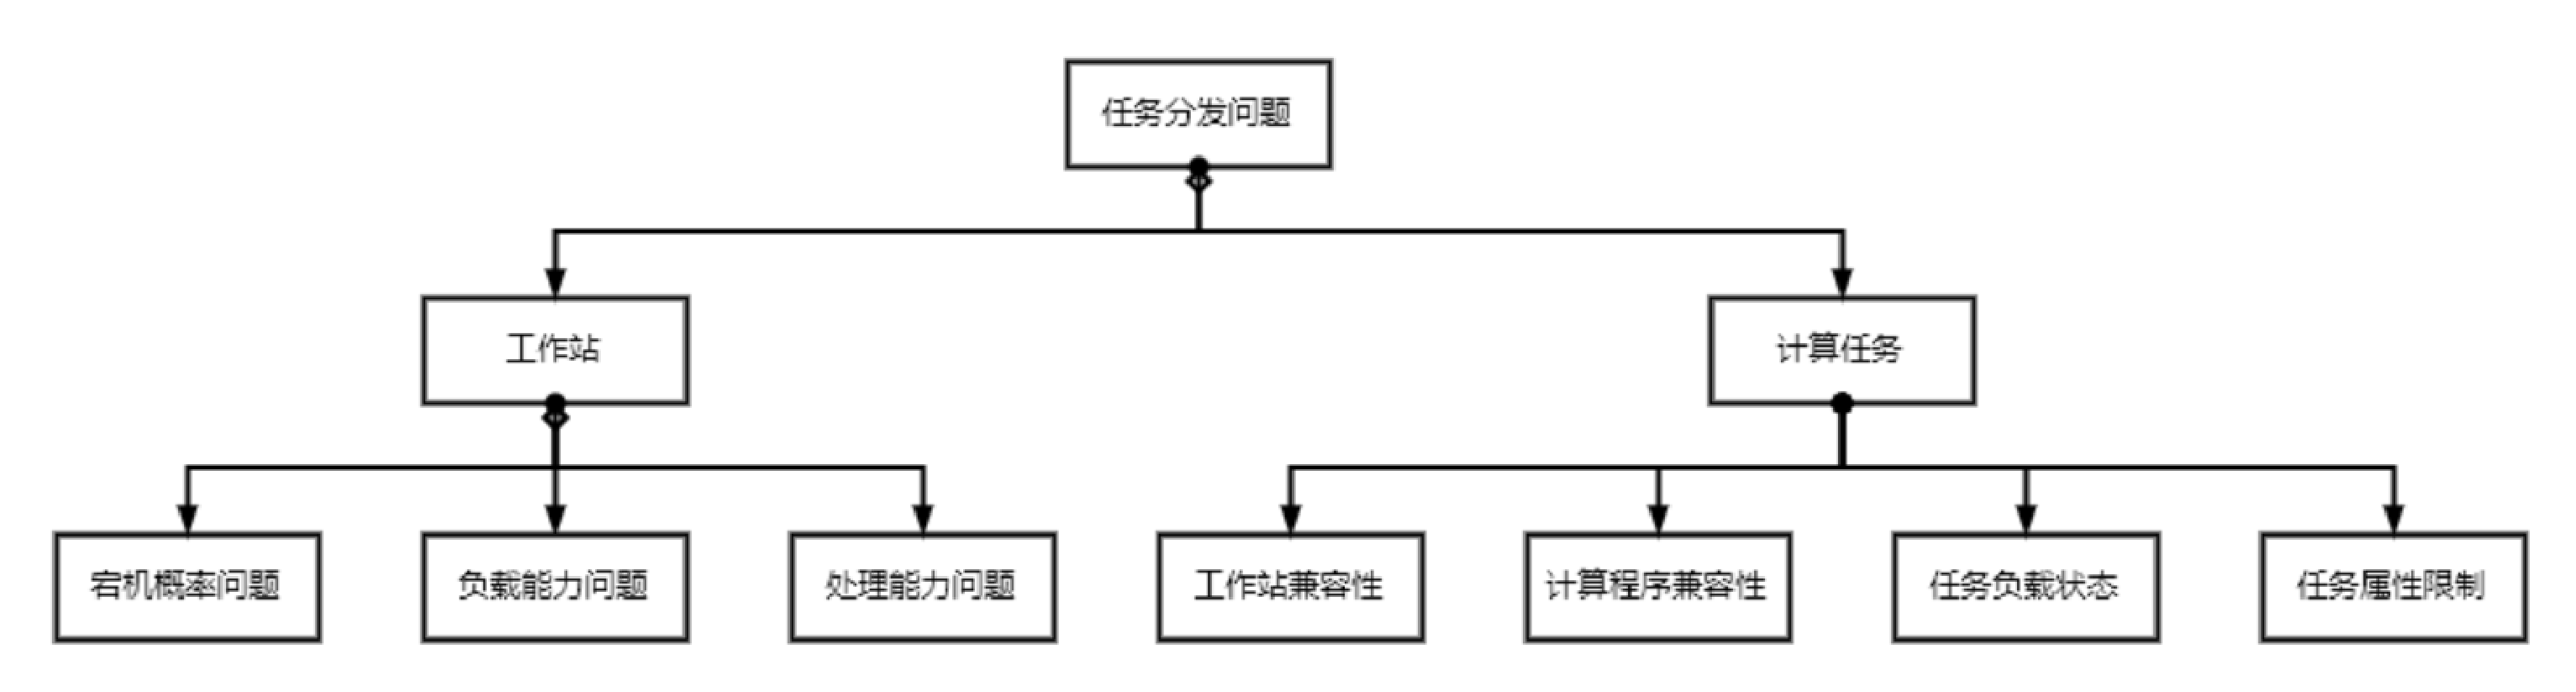
\includegraphics[width=0.80\textwidth]{1.1.eps} %中间那个是设置图片的宽度(文本行的0.8倍)
	\centering
  	\caption{问题一分析图解}%设置名字
	\end{figure}

	\subsection{问题一的分析}
任务分发的关键点在于工作站端和计算任务端,这两个方面的限制直接影响了任务分发的成效,因此如何去量化这些两个方面的关键指标,以及如何去组合任务分配,是任务分发需要解决的问题。

\subsubsection{工作站端的问题}

\bf{宕机概率问题}

工作站在处理趋近自己能力上限的一组计算任务时有一定几率会发生宕机,当超过能力上限的时候一定会发生宕机。宕机时工作站的计算会失败。根据工作站宕机的这一特性,要求我们在分配任务的时候搭配好每一台工作站的任务量,使得宕机的情况尽量不发生。此外,我们还需要平衡宕机的概率和任务量之间的关系,使之保持在一个较为均衡的状态。我们可以知道,计算任务所需要的能力越高,越容易导致宕机,因此可以使用分段函数来描述任务量和宕机概率的关系。

\bf{负载能力问题}

根据分布式网络计算的定义,每一个工作站所接受到的任务数量(含执行的任务数量)即这个工作站的负载。对于每个工作站而言,在没有某些特殊任务执行的时候,他的最大负载是恒定的,对于超出负载的任务无法执行。因此在分配任务时分配任务的数量应该保持在合理的范围之中。当负载为0时,工作站没有处理任何任务,其资源被浪费;而当负载超过上限的时候,超过部分就不会被执行,同样会造成浪费。

这里需要说明负载和任务量的关系:对于工作站而言,任务量的大小取决于任务的某一属性,任务量的总和会影响到宕机的概率;而负载则是一个绝对的数量,只和任务的数量有关,任务的数量超过工作站的最大负载时,工作站也不会执行更多程序。

\bf{处理能力问题}

对于工作站而言,由于CPU,内存,网络带宽等因素,其处理计算任务的能力有一定的差异,而每个计算任务由于其复杂度的差别,任务量有所不同,对于这一能力的需求也有不同。在分配任务时,一工作站的任务量应当不超过处理能力的最大值,否则在超过工作站的处理能力时发生宕机,导致运算失败,较之于不宕机的分配方式是一种对于计算资源的不合理分配。

\subsubsection{计算任务的问题}

\bf{工作站兼容性}

由于某些限制,有些计算任务不能发布在某些工作站上,这要求我们把是否需要特定分配工作站和需要分配哪些工作站记录在任务的属性中。在进行分配设计的时候进行适配。

\bf{计算程序的兼容性}

由于实际运用的需要,某些计算程序需要在同一个工作站中运行,而有的计算程序一定不能在同一工作站中运行。计算程序的兼容性也需要记录在任务属性中。分配时将必须在一起的分到相同的工作站,对于那些不能同时运行在同一个工作站上的,就将他们分开。

\bf{任务负载状态}

某些特殊的计算程序会影响到其所在工作站的负载能力。当这些计算程序的数量到达某个阈值的时候,工作站的最大负载能力会有所减弱,减弱的值是一个常数。这样的特殊程序需要尽量控制在阈值之内以免影响工作站的负载能力,除非在超出阈值后得到整体的优化,才会采取超出阈值的策略。

\bf{任务属性限制}

每个任务由于其算法和复杂度的不同,带来了不同的工作量,我们使用任务属性值这一指标来量化分析不同计算任务的工作量。这里就可以同工作站在宕机概率问题和处理问题中的工作量联系起来,进而进行量化的分析,求出最佳的分配方案。

\subsubsection{非线性规划模型}

在分析完工作站和计算任务的属性及其限制条件之后,我们就可以进行非线性规划,寻求最佳的分配方式。在这个非线性规划中,约束条件是基于工作站的宕机概率,负载能力和处理能力,以及任务的兼容性,负载状态和属性限制进行设定。最优化的指标有以下两个方面:(1)工作站的总期望返回值;(2)已经分配的任务属性值之和。这将在后续模型建立的过程中进行分析。

	\section{模型假设}

同时运行

由于工作站的CPU是多线程处理器,可以在同一时刻内进行多个程序的处理,一组程序被分发到同一个工作站运行即被视为同时运行。

处理能力

假设每个工作站的处理能力上限和计算程序的处理能力要求可以按照某一方法量化。

对于工作站而言,由于CPU,内存,网络带宽等因素,其处理计算任务的能力有一定的差异,而每个计算程序由于其复杂度的差别,任务量有所不同,对于这一能力的需求也有不同。为了把这些软硬件问题抽象出来,我们使用一个数学符号$W$来进行量化。

与之对应的是计算任务对于处理能力需求的量化,这一需求我们使用一符号$v$表示。这样就可以线性组合各个任务对于能力的需求,使之在不超过工作站处理能力上限的同时,满足全局的最优化。

宕机的概率分布

假设每个工作站宕机的概率分布是关于此工作站使用能力$\sum_{T_{i}\in S_j}v_i$的分段函数。并使用参数$\sigma$来描述函数关系的不确定性。

由计算机的处理能力可知,在工作站使用能力趋于其上限时,使用能力和其宕机概率成正相关。由于实际因素的影响,这种相关性的具体分布未知,为此我们使用一个正比例函数加上一个随机量$\sigma$来表示这样的不确定性关系。

属性值

假设每一个计算任务所返回的属性值就是其需要的处理能力要求。

这一假设的目的在于量化计算任务的执行状态和任务处理能力需求的关系,以期通过建立返回值的期望函数模型,来评估整个分配方案的优劣。

数量关系的假设

1.计算任务的数量大于工作站的数目

2.每个工作站的最大负载一致





	\section{变量说明}

\begin{center}
		\begin{tabularx}{0.8\textwidth}{c@{\hspace{1pc}}|@{\hspace{2pc}}X}

			\Xhline{0.08em}
			符号 & \multicolumn{1}{c}{符号说明}\\
			\Xhline{0.05em}
		​	$m$ & 工作站数目\\

​			$n$ & 计算任务数目\\

​			$T_i=(\alpha_i,\beta_i,v_i,l_i)$ & 第$i$个计算任务的参数\\

​			$\alpha_i$ & 计算任务$i$的工作站兼容参数 \\

​			$\beta_i$ & 计算任务$i$的其他任务兼容参数\\

​			$v_i$ & 计算任务 $i$的属性值\\

			$l_i$ & 计算任务$i$的负载系数\\

​			$S_i=(W_{imax},R_0,L_i,k_i)$ & 第$iC$个工作站的参数\\

​			$W_{imax}$ & 第$i$台工作站的最大处理能力\\

			$L_i$ & 第$i$台工作站的负载能力\\

			$P$ & 工作站的阈值\\

			$k_i$ & 工作站超过阈值后的负载衰减常数\\
​
​			$_i$ & 工作站$S_i$的总返回值  \\

			$_i$ & 工作站$S_i$的总期望返回值\\

			$R_0$ & 工作站$_i$的宕机概率系数\\

			$\sigma$ & 工作站宕机概率偏移量\\

​			$E$ & 工作站的总返回值\\

			$O$ & 已经分配的任务属性值之和\\
			\Xhline{0.08em}
		\end{tabularx}
	\end{center}




	\section{模型建立与求解}
\subsection{问题一模型的建立}

在前述的问题分析中,每一个计算任务和工作站都有已知的参数,我们使用由数个参数组成的向量来描述整个计算任务或是工作站的属性。

\subsubsection{计算任务的参数说明}
\begin{equation}
T_i=(\alpha_i,\beta_i,v_i,l_i)
\end{equation}


1.$\alpha_i$是每一个计算任务的工作站兼容参数。

此参数是一个$1\times m$的列向量,由数字0和1构成
\begin{equation}
\alpha_i=(0,1,0,0,0,\dots,0,1,0)^T
\end{equation}
第$i$个元素的数值表示计算程序对于此工作站的兼容性,0代表可以运行于此工作站,1代表不能运行于此工作站。

2.$\beta_i$用于识别计算任务$T_i$与其他任务的兼容性,对于一个必须同时在同一工作站执行任务组:
\begin {equation}
A=\{T_1,T_2,T_3,\dots\},|A|<L_0
\end{equation}
有$\forall T_i\in A,\beta_i$是一个相等且唯一的值,与每一个任务组唯一对应。不同的任务组有不同的唯一$\beta$与之对应。当一个任务组必须同时运行在同一个工作站时,$\beta>0$,一个任务组一定不能同时运行,$\beta<0$,其余的任务的$\beta=0$.


% Table generated by Excel2LaTeX from sheet 'Sheet1'
\begin{table}[htbp]
  \centering
    \begin{tabular}{ll}
\Xhline{0.08em}
    $\beta$       &  兼容性  \\
\Xhline{0.08em}
      $\beta>0$     &  必须和任务组中的元素运行于同一个工作站 \\
      $\beta=0$     & 没有特殊要求  \\
      $\beta<0$      & 一定不能和任务组中的其余所有元素运行于同一个工作站 \\
\Xhline{0.08em}
    \end{tabular}%
  \caption{任务兼容性与$\beta $的关系}
  \label{tab:addlabel}%
\end{table}%


3.计算任务$i$的属性值$v_i$

在前文的描述中,计算任务$t_i$对于处理能力需求的量化使用$v_i$来表示,每个任务的复杂度,内存占用和算力占用被统一量化形成该指标。使用这一抽象的指标化简问题,并且在后续的返回值处理中创造判据。

4.计算任务$T_i$的负载系数$l_i$

负载系数是一个布尔值,有0和1两个状态。如果某计算任务的这一数值是0,那么就不会对$L_i$产生影响,当计算任务的这一数值为1,并且在某个工作站中$l_i$为1的计算任务数量超出某个阈值$P$时,工作站负载能力会有常数$k_i$的衰减。

\subsubsection{工作站的参数说明}
\begin{equation}
S_i=(W_{imax},R_0,L_i,k_0)
\end{equation}

1. 第$i$台工作站的最大处理能力$W_{imax}$

工作站的最大处理能力直接限制一次所能处理的计算任务属性值之和。若计算任务属性值之和超过工作站的最大处理能力,工作站发生宕机,这对工作效率是不利的影响。经后文对数学期望的计算,我们可知应一定要使计算任务属性值之和不大于工作站的最大处理能力。

2.工作站$m_i$的宕机概率系数$R_0$ 与 工作站宕机概率偏移量$\sigma$ 
 
工作站的宕机概率系数$R_0$以及宕机概率偏移量$\sigma$,会影响工作站在未达到最大处理状态发生宕机的概率,从而影响到工作站返回值数学期望的计算。我们定义:在工作站恰好达到最大处理状态时,发生宕机的概率为$R_0$+$\sigma$。($\sigma$是一与属性值之和相关的未知量)

3.第$i$台工作站的负载能力$L_i$ 
 
工作站的负载能力会限制其能处理的计算任务的数量,从而限制该工作站处理的计算任务属性值之和,影响工作站的运行效率。当前文所述$l_i$为1的计算任务数量超出某个阈值$P$时,工作站负载能力会有常数$k_i$的衰减。此时工作站需要剔除某几个计算任务,从而影响返回值的期望$E$,以及目标的剩余总返回值$O$.我们将在在后续模型求解中考虑这一因素。

4.工作站超过阈值后的负载衰减常数$k_i$  

负载衰减常数只与工作站本身的属性有关,与特殊计算任务的数量,属性值之和等因素无关。由3.可知,在特殊计算任务的数量超过阈值时,负载衰减常数也会影响工作站的运行效率。


\subsubsection{目标函数的求解}

为了反映工作站的运行效率,我们采用一个目标函数来计算,且该目标函数的值与工作站的运行效率成正相关。该目标函数由两部分组成:工作站的总返回值E和所有计算任务属性值之和$V_i$。即两者按一定的权重$\omega_1,\omega_2$对目标函数的值做出贡献。
\begin{equation}
\Large F=\omega_1 E+\omega_2O\label{zz1}
\end{equation}
对工作站的总返回值E有
\begin{equation}
\Large E=\sum_{j=1}^{m} C_j\label{zz2}
\end{equation}
对上式的推导过程如下:

先只考虑一个工作站的返回值期望$C_j$
\begin{equation}
\large C_j =V_i(1-f(V_i))\label{zz3}
\end{equation}
下面是对于工作站返回值期望的具体分析

$C_j$由$V_i$和$f()$确定,$V_j$是工作站的总返回值,含义是分配到每个工作站的计算任务($V_i \in S_j$)属性值之和,计算公式如下:
\begin{equation}
\large V_j=\sum_{v_i \in S_j}v_i\label{zz4}
\end{equation}
由题设可知,一个工作站宕机的情况分为两种:其一为该工作站上计算任务属性值之和$V_i$超过了工作站的最大处理能力$W_{imax}$,此情况下宕机概率为100\%;其二为该工作站上计算任务属性值之和$V_i$不超过工作站的最大处理能力$W_{imax}$,此时有一定概率$f(V_i)$发生宕机,且与计算任务$f(V_i)$和工作站的属性配置相关。

第一种情况较为简单,即$V_i$>$W_{imax}$时,$f(V_i)$=100\%

现研究第二种情况下$f(V_i)$的表达:

根据题意与计算机,$f(V_i)$与计算任务和工作站的属性配置有相关,无法具体确定,因此我们可以将$f(V_i)$分为两部分讨论,即$f(V_i)= g(V_i)+\sigma$,一部分$g(V_i)$由与计算任务和工作站的属性配置确定,另一部分由宕机概率偏移量$\sigma$随机生成,且$\sigma$也与计算任务和工作站的属性配置相关。

我们假设,第一部分g($V_i$)与计算任务属性值之和$V_i$成正比,与工作站的最大处理能力$W_{imax}$成反比,同时考虑宕机概率系数$R_0$可得:
\begin{equation}
\Large g(V_i)= R_0\frac{V_i} {W_{imax}}\label{zz5}
\end{equation}
第二部分为
\begin{equation}
\Large\sigma=h·\frac{V_i}{W_{imax}}\label{zz6}
\end{equation}
$h$为随机生成数字,在区间10\%-20\%,反映了$f(V_i)$的不确定性。

故有
\begin{equation}
\Large f(V_i)=(R_0+h)\frac{V_i} {W_{imax}}\label{zz7}
\end{equation}
分析可知,对某一特定的工作站,$W_{imax}$一定,计算任务属性值之和$V_i$越大,发生宕机概率越大;同理,对一定的计算任务属性值之和$V_i$,工作站的最大处理能力$W_{imax}$越大,发生宕机的概率越小,符合实际情况。

综上所述结合(6)(7)(8)(9)(10)(11)式,我们可以得出函数关系

\begin{equation}\large
f(V_i) = \begin{cases}
1, & V_i>W_{imax} \\
 (R_0+h)\frac{V_i} {W_{imax}}, & V_i\leq W_{imax} \\
\end{cases}  \label{zz8}
\end{equation}

下面进行已分配任务属性值之和$O$的计算

已分配任务的属性值之和$O$为各个工作站的总返回值$V_i$之和。要注意在计算过程中总返回值$V_i$是对于分配在此工作站上任务属性值$v_i$的求和,而非总期望返回值$C_i$。
\begin{equation}
\large O=\sum_{j=1}^mV_j
\end{equation}
将工作站的总期望返回值和,已经分配的属性值之和计算完毕之后,根据处理实际问题中的偏向有所不同,我们使用一定的数量关系进行两个指标的权重分配。对于权重$\omega_1,\omega_2$有以下说明:

(1)两个指标数量关系的约束:$\omega_1+\omega_2=1$

(2)在分布式运算的处理过程中,对于任务处理评价的指标具有两方面要求:稳定性的要求和对于算力分配的需求。在一个稳定性强的分布式运算架构中,工作站的异常状态(在本例中只考虑了宕机)对计算任务的影响应当尽可能的小。也就是说,在处理一组算力需求相同的计算任务时,如何分配任务从而使得工作站的异常状态对于计算任务的影响最小,是规划的指标之一。与此同时,一些工作站对于任务的需求是利用有限的资源处理最多的运算量,使得运算的资源达到最佳利用。

容易看出,这两个指标每一个单独探讨都是没有意义的。单纯追求分布式运算的稳定性会带来算力资源的极大浪费,只考虑算力最优分配就会导致系统宕机概率增加,减少稳定性。通过引入系数$\omega_1,\omega_2$调整侧重,可以获得全局的最优解决方案。

\subsubsection{对于影响工作站最大负载计算程序的考虑}

在前文的描述中引入了某些影响工作站最大负载的计算程序,这些计算程序的负载系数都是1,当数量超过阈值的时对于工作站的最大负载有常数上的衰减。由于在工作站最大负载较之于衰减系数是一个较大的值,这样的衰减可以忽略不计,从而工作站的处理能力使用量的变化也可以忽略不计,进而也几乎不会对宕机概率的分布产生影响,这样对于整体取得最优化没有影响。因此,我们在规划的构建过程中,并未将衰减纳入考虑。

\subsection{问题一模型的建立}

\subsubsection{创建分配矩阵和兼容属性矩阵}

​(1)分配矩阵

对于每一个计算任务的分配方式,可以通过一个$m\times n$的0-1矩阵来表示出分配的关系
\begin{equation}
{\begin{bmatrix}0&1&\cdots&\cdots&\cdots&1\\1&\ddots&&&\vdots&0\\0&\cdots&a_{ij}&&\vdots&0\\&&\cdots&\cdots&&\\0&1&0&0&0&1\\\end{bmatrix}}_{m\times n}
\end{equation}
元素$a_{ij}$为1的含义是任务$T_j$被分配到工作站$S_i$上,为0的含义就是任务$T_j$不可以被分配到工作站$S_i$上。这一矩阵是我们求解的目标,借此可以利用MATLAB或LINGO把这一矩阵输入,进行线性或是非线性规划。由于每个任务只能被分配一次,故分配矩阵每一列的元素和小于等于1.

(2)任务兼容矩阵

对每一个计算任务与其他任务的兼容性,每一个任务的兼容性有一个其他任务兼容参数$\beta$进行描述。不同的任务组有不同的唯一$\beta$与之对应。当一个任务组必须同时运行在同一个工作站时,$\beta>0$,一个任务组一定不能同时运行,$\beta<0$,其余的任务的$\beta=0$.在进行计算机求解的时候,所有任务$T$的$\beta$的具体数值被处理为一个对称0-1矩阵,如下图所示:
\begin{equation}
{\begin{bmatrix}1&1&\cdots&\cdots&\cdots&-1\\1&\ddots&&&\vdots&0\\0&\cdots&a_{ij}&&\vdots&0\\&&\cdots&\cdots&&\\-1&1&0&0&0&1\\\end{bmatrix}}_{n\times n}
\end{equation}
该对称矩阵有以下几个性质:


\begin{enumerate}
\item 只由-1,0,1组成,$a_{ij}$为1时任务$T_i$与$T_j$一定同时运行,$a_{ij}$为-1时任务$T_i$与$T_j$一定不能同时运行,$a_{ij}$为0时任务$T_i$与$T_j$运行互不影响。

\item$a_{ij}=a{ji}$,兼容关系具有相互性,不允许两个元素间有不同的兼容状态

\item 规定:对角线上的元素都是1

在进行处理时,可以按照矩阵的运算性质判定任务的分发方案是否满足了任务兼容的约束指标

(3)工作站兼容矩阵
\end{enumerate}
在问题分析中我们引入计算任务$T$的工作站兼容参数$\alpha$,此参数是一个$1\times m$的行向量,由数字0和1构成

\begin{equation}

\alpha_i=(0,1,0,0,0,\dots,0,1,0)^{T}

\end{equation}

第$i$个元素的数值表示计算程序对于此工作站的兼容性,0代表可以运行于此工作站,1代表不能运行于此工作站。

我们将每个任务$T$进行组合,构成一个$m\times n$的0-1矩阵来表示任务总体的兼容关系
\begin{equation}
{\begin{bmatrix}\alpha_1&\alpha_2&\alpha_3&\cdots&\alpha_n\\\end{bmatrix}}={\begin{bmatrix}0&1&\cdots&\cdots&\cdots&0\\1&\ddots&&&\vdots&0\\0&\cdots&a_{ij}&&\vdots&0\\&&\cdots&\cdots&&\\0&1&0&0&0&1\\\end{bmatrix}}_{m\times n}
\end{equation}
元素$a_{ij}$为1的含义是任务$T_j$不能被分配到工作站$S_i$上,为0的含义就是任务$T_j$可以被分配到工作站$S_i$上。该矩阵在初始情况下就已经确定。


















\section{使用图像}
\begin{figure}[h]%参数h代表在当前位置加入图像
	\centering
	
\includegraphics[width=0.80\textwidth]{2021-04-01_202009.eps} %中间那个是设置图片的宽度(文本行的0.8倍)
	\centering
  	\caption{mou tai chou}%设置名字

\end{figure}
注意文件需要放在figure文件架里面,而且需要转化成eps格式(使用那个批处理)
https://zhuanlan.zhihu.com/p/32925549 这个是关于多个图像并排搞得问题
	\subsection{问题1}
\begin{equation}
\oiint  \label{XX}
\end{equation}

\begin{equation}
		 \label{yy}
\end{equation}

\begin{equation}
{\begin{bmatrix} 0 & 0 &\cdots & \cdots & 0\\ 1-d_{i_1}(t) & 0 & 0 &0 & \vdots\\0&1-d_{i_2}(t)&0&0&\ddots \\\ddots&\vdots&\vdots& &0\\\end{bmatrix}}_{m n}
\end{equation}

\begin{equation}
D(x) = \begin{cases}
\lim\limits_{x \to 0} \frac{a^x}{b+c}, & x<3 \\
\pi, & x=3 \\
\int_a^{3b}x_{ij}+e^2 \mathrm{d}x,& x>3 \\
\end{cases}  \label{zz}
\end{equation}

\begin{equation}
\lim_{x \to \infty} x^2_{22} - \int_{1}^{5}x\mathrm{d}x + \sum_{n=1}^{20} n^{2} = \prod_{j=1}^{3} y_{j}  + \lim_{x \to -2} \frac{x-2}{x}  \label{pp}
\end{equation}

\begin{equation}
\overbrace{1+2+\cdots+n}^{n个} \qquad \underbrace{a+b+\cdots+z}_{26}  \label{qq}
\end{equation}


	\subsubsection{content}
\centering 
how to slove this problen ?\newline


	\subsection{问题12}
	\subsubsection{content}
	\subsection{问题3}
	\subsubsection{content}
	\subsection{问题4}
	\subsubsection{content}

	\section{模型评价与推广}
	\subsection{模型优点}
	\subsection{模型缺点}
	


	\newpage

	\phantomsection
	\addcontentsline{toc}{section}{参考文献}

	\begin{thebibliography}{99}
	\bibitem{label}content
	复制内容在这里
	\bibitem{label}content
	复制内容在这里
	\end{thebibliography}

	\newpage
	\appendix
	\ctexset{section={
		format={\zihao{-4}\heiti\raggedright}
	}}
	\begin{center}
		\heiti\zihao{4} 附\hspace{1pc}

	\end{center}
	\section{附录一:的娃娃的}
	阿瓦吊带袜
	\section{附录二:的娃娃的}
	阿瓦吊带袜
	测试列表
\begin{itemize}
\item 无编号的列表
\item 带编号的列表
\item 带标签的列表
\end{itemize}

\begin{enumerate}
\item 无编号的列表
\item 带编号的列表
\item 带标签的列表
\end{enumerate}



\end{document}